\begin{figure}
	\centering
	\setlength{\imagewidth}{0.8\textwidth}%
	\setlength{\imageheight}{0.85\imagewidth}%
	%
	\DTLsetseparator{,}%
	\DTLloaddb[noheader,keys={x,y}]{dbvertex}{figures/data/pseudo_EdS_sommet/trimmed_patch/xy_vertex.dat}%
	\DTLloaddb[noheader,keys={x,y,tx,ty}]{dbplanes}{figures/data/pseudo_EdS_sommet/trimmed_patch/xy_planes.dat}%
	\DTLloaddb[noheader,keys={r,g,b}]{dbcolorplanes}{figures/data/pseudo_EdS_sommet/trimmed_patch/color_planes.dat}%
	\DTLloaddb[noheader,keys={x,y,l}]{dbcorners}{figures/data/pseudo_EdS_sommet/trimmed_patch/xy_corners.dat}%
	%
	\pgfmathtruncatemacro\nfaces{\DTLrowcount{dbplanes}}
	%
	\begin{tikzpicture}[
		x=\imagewidth,
		y=\imageheight,
		img/.style={anchor=south west, inner sep=0},
		curv/.style={line width=0.8pt, line cap=round},
		vector/.style = {-latex', thick},
		label/.style = {font=\small},
		labelpoint/.style = {font=\normalsize},
		insert node/.style args={#1 at #2 raised #3}{
    		postaction=decorate,
    		decoration={
      			markings,
      			mark = at position #2 with {#1},
      			raise = #3
      		}
		}
	]
	%
	\DTLassign{dbvertex}{1}{\vx=x, \vy=y}%
	%
	\begin{scope}
		%
%		\begin{scope}[blend group = color]
%			{\transparent{0.5}%
%				\node[img] at (0,0) {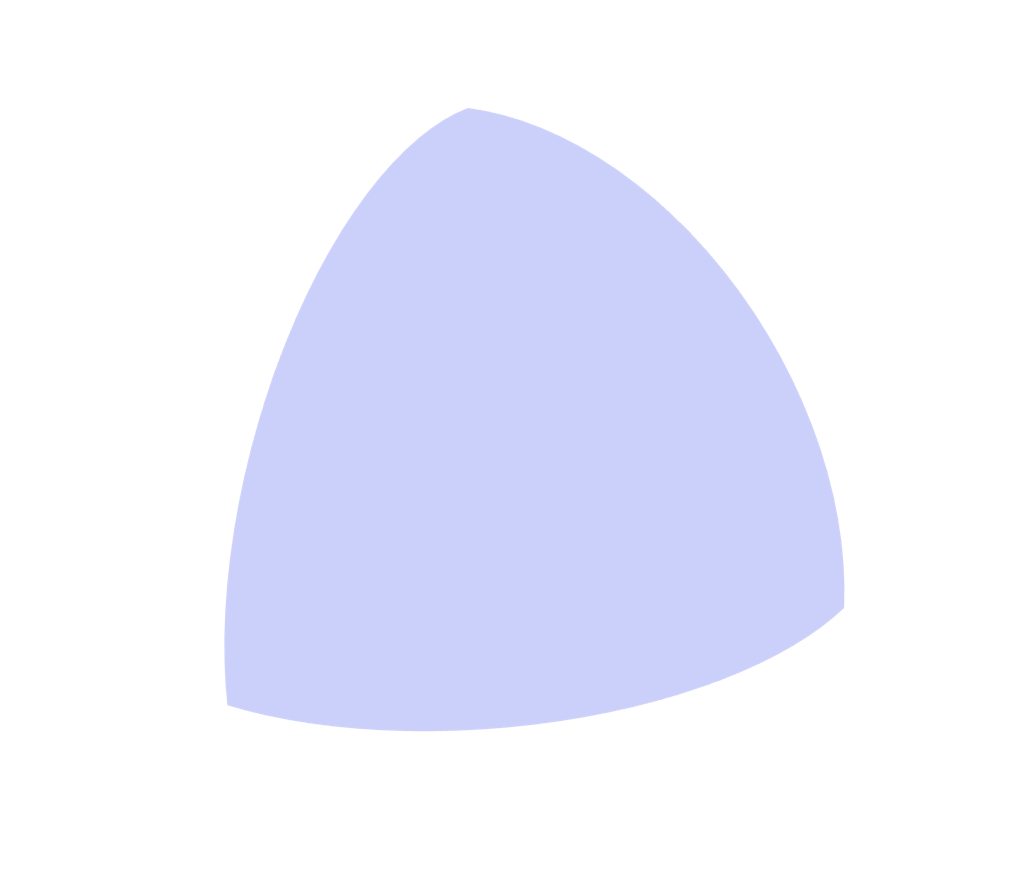
\includegraphics[width=\imagewidth]{pseudo_EdS_sommet/trimmed_patch_shadeless_only}};
%			}%
%			\node[img] at (0,0) {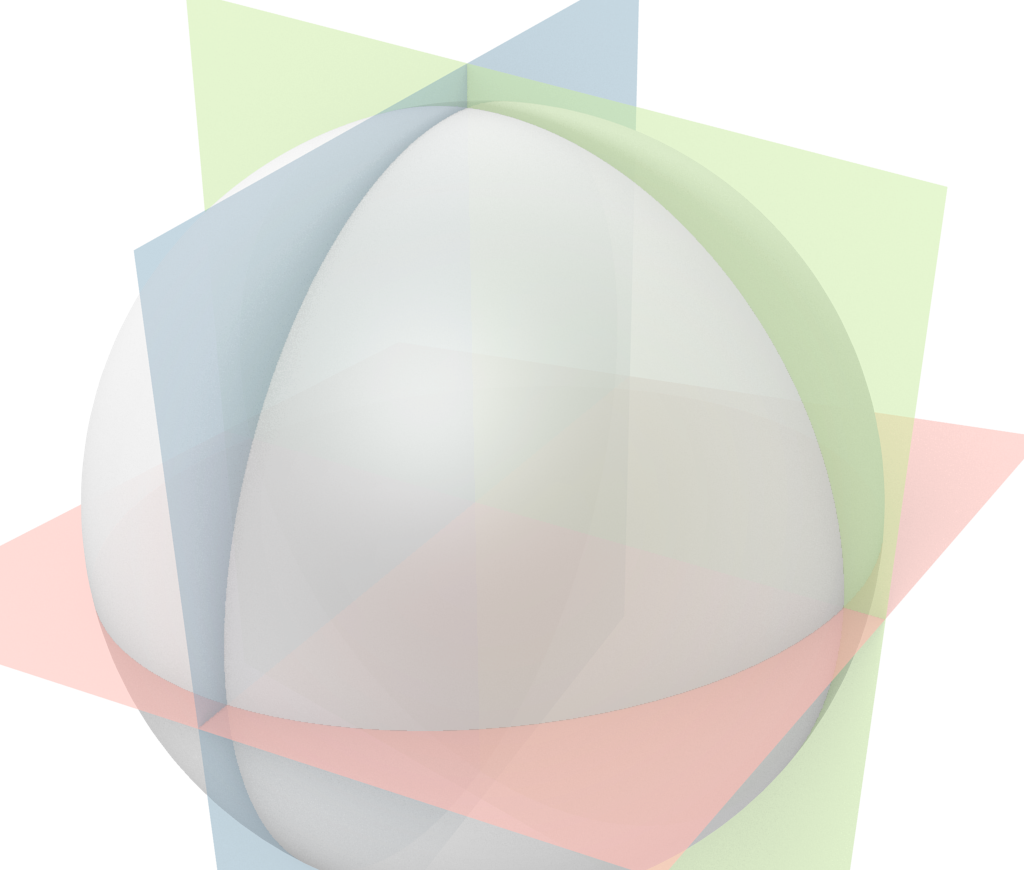
\includegraphics[width=\imagewidth]{pseudo_EdS_sommet/sphere_planes}};
%		\end{scope}
		\node[img] at (0,0) {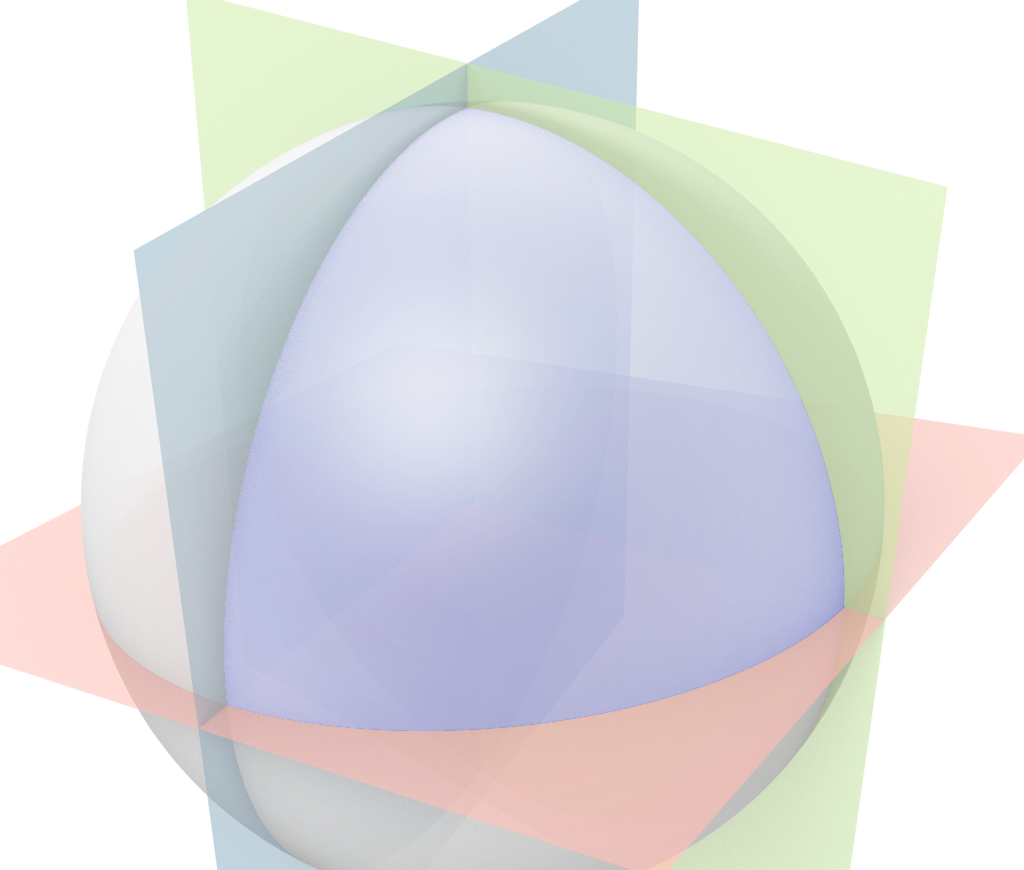
\includegraphics[width=\imagewidth]{pseudo_EdS_sommet/sphere_planes_trimmed_patch}};
		%
		\DTLforeach{dbplanes}{\ox=x, \oy=y, \tx=tx, \ty=ty}%
		{%
			%
			\DTLassign{dbcolorplanes}{\arabic{DTLrowi}}{\pcolorr=r, \pcolorg=g, \pcolorb=b}%
			\definecolor{planecolor}{rgb}{\pcolorr, \pcolorg, \pcolorb}
			\colorlet{circlecolor}{planecolor!80!black}
			%
			\pgfmathtruncatemacro\iplane{\arabic{DTLrowi} - 1}
			%
			{\transparent{0.5}%
				\draw[curv, dash pattern=on 2pt off 4pt, circlecolor] plot file {figures/data/pseudo_EdS_sommet/trimmed_patch/xy_arc_dashed_\iplane.dat};
			}%
			\draw[curv, circlecolor] plot file {figures/data/pseudo_EdS_sommet/trimmed_patch/xy_arc_solid_\iplane.dat};
			%
			\fill[circlecolor] (\ox, \oy) circle (1.2pt);
			\draw[
				circlecolor,
				vector,
				insert node={\node[labelpoint, circlecolor] {$\lo{\bo}_{\iplane}$};} at 0.06 raised -1.4ex,
			] (\ox, \oy) -- (\tx, \ty) node[pos=1.09] {$\lo{\bt}_{\iplane}$};
		}%
		%
		\fill[black] (\vx, \vy) circle (1.35pt);
		\node[labelpoint] at ([shift={(145:5pt)}]\vx, \vy) {$\v$};
		%
		\DTLforeach{dbcorners}{\nx=x, \ny=y, \nl=l}%
		{%
			%\pgfmathtruncatemacro\iplane{\arabic{DTLrowi} - 1}
			%
			\draw[vector] (\vx, \vy) -- (\nx, \ny) node[pos=1.07] {$\nl$};
			%\fill[black] (\nx, \ny) circle (1.2pt);
		}%
		%
	\end{scope}
	%
	\end{tikzpicture}
	\DTLgdeletedb{dbvertex}%
	\DTLgdeletedb{dbplanes}%
	\DTLgdeletedb{dbcolorplanes}%
	\DTLgdeletedb{dbcorners}%
	%
	\caption{Représentation de la pseudo-EdS d'un sommet à l'aide d'un seul carreau restreint.}
	\label{fig:pseudo_EdS_sommet_trimmed_patch}
\end{figure}